%!TEX root =  ../guia-MD.tex

\chapter{L�gica Proposicional}

\section*{Prepare-se!}

Nesta aula, estudaremos os conceitos b�sicos sobre assunto.

Antes desta aula, o estudante deve ler o livro texto da disciplina \cite{rosen09}.

\section*{Notas de Aula}

\begin{minipage}{0.7\linewidth}

Inserir  notas de aula. Inserir  notas de aula. Inserir  notas de aula. Inserir  notas de aula. Inserir  notas de aula. Inserir  notas de aula. Inserir  notas de aula. Inserir  notas de aula. Inserir  notas de aula. Inserir  notas de aula. Inserir  notas de aula. Inserir  notas de aula. 

Inserir  notas de aula. Inserir  notas de aula. Inserir  notas de aula. Inserir  notas de aula. Inserir  notas de aula. Inserir  notas de aula. Inserir  notas de aula. Inserir  notas de aula. Inserir  notas de aula. Inserir  notas de aula. Inserir  notas de aula. Inserir  notas de aula. Inserir  notas de aula. Inserir  notas de aula. Inserir  notas de aula. Inserir  notas de aula. Inserir  notas de aula. Inserir  notas de aula. Inserir  notas de aula. Inserir  notas de aula. Inserir  notas de aula. Inserir  notas de aula. Inserir  notas de aula. Inserir  notas de aula. Inserir  notas de aula. Inserir  notas de aula. Inserir  notas de aula. Inserir  notas de aula. Inserir  notas de aula. Inserir  notas de aula. Inserir  notas de aula. Inserir  notas de aula. Inserir  notas de aula. Inserir  notas de aula. Inserir  notas de aula.

Como na Figura \ref{fig:type}

Inserir  notas de aula. Inserir  notas de aula. Inserir  notas de aula. Inserir  notas de aula. Inserir  notas de aula. Inserir  notas de aula. Inserir  notas de aula. Inserir  notas de aula. Inserir  notas de aula. Inserir  notas de aula. Inserir  notas de aula. Inserir  notas de aula. Inserir  notas de aula. Inserir  notas de aula. Inserir  notas de aula. Inserir  notas de aula. Inserir  notas de aula. Inserir  notas de aula. Inserir  notas de aula. Inserir  notas de aula. Inserir  notas de aula. 

Teste acentos. Computa��o. L�gica.

\end{minipage}

\begin{figure}[htbp]
\begin{center}
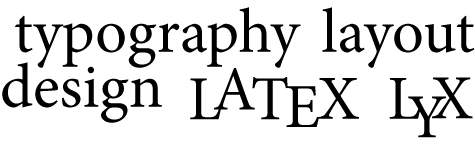
\includegraphics[scale=0.4]{aulas/figuras/type.png}
\caption{Teste.}
\label{fig:type}
\end{center}
\end{figure}


\newpage
\section*{Exerc�cios de Fixa��o}

\begin{enumerate}
\item $P = NP$ ?
\item Qual a l�gica do universo e todas as coisas al�m?
\end{enumerate}